\subsection{Novel Feedback Configurations}
The main objective of the study was to evaluate the effectiveness of two novel electrotactile feedback configurations in providing proprioceptive information of a two DoF myoelectric prosthesis. 
The DoF's used were wrist rotation and hand aperture. The transmitted feedback was discrete, where the full range of each feedback variable was been divided into five segments. The electrode array used to deliver electrical stimulation can be seen in figure \ref{fig:pa:electrode}.
\begin{figure}[H]                 
	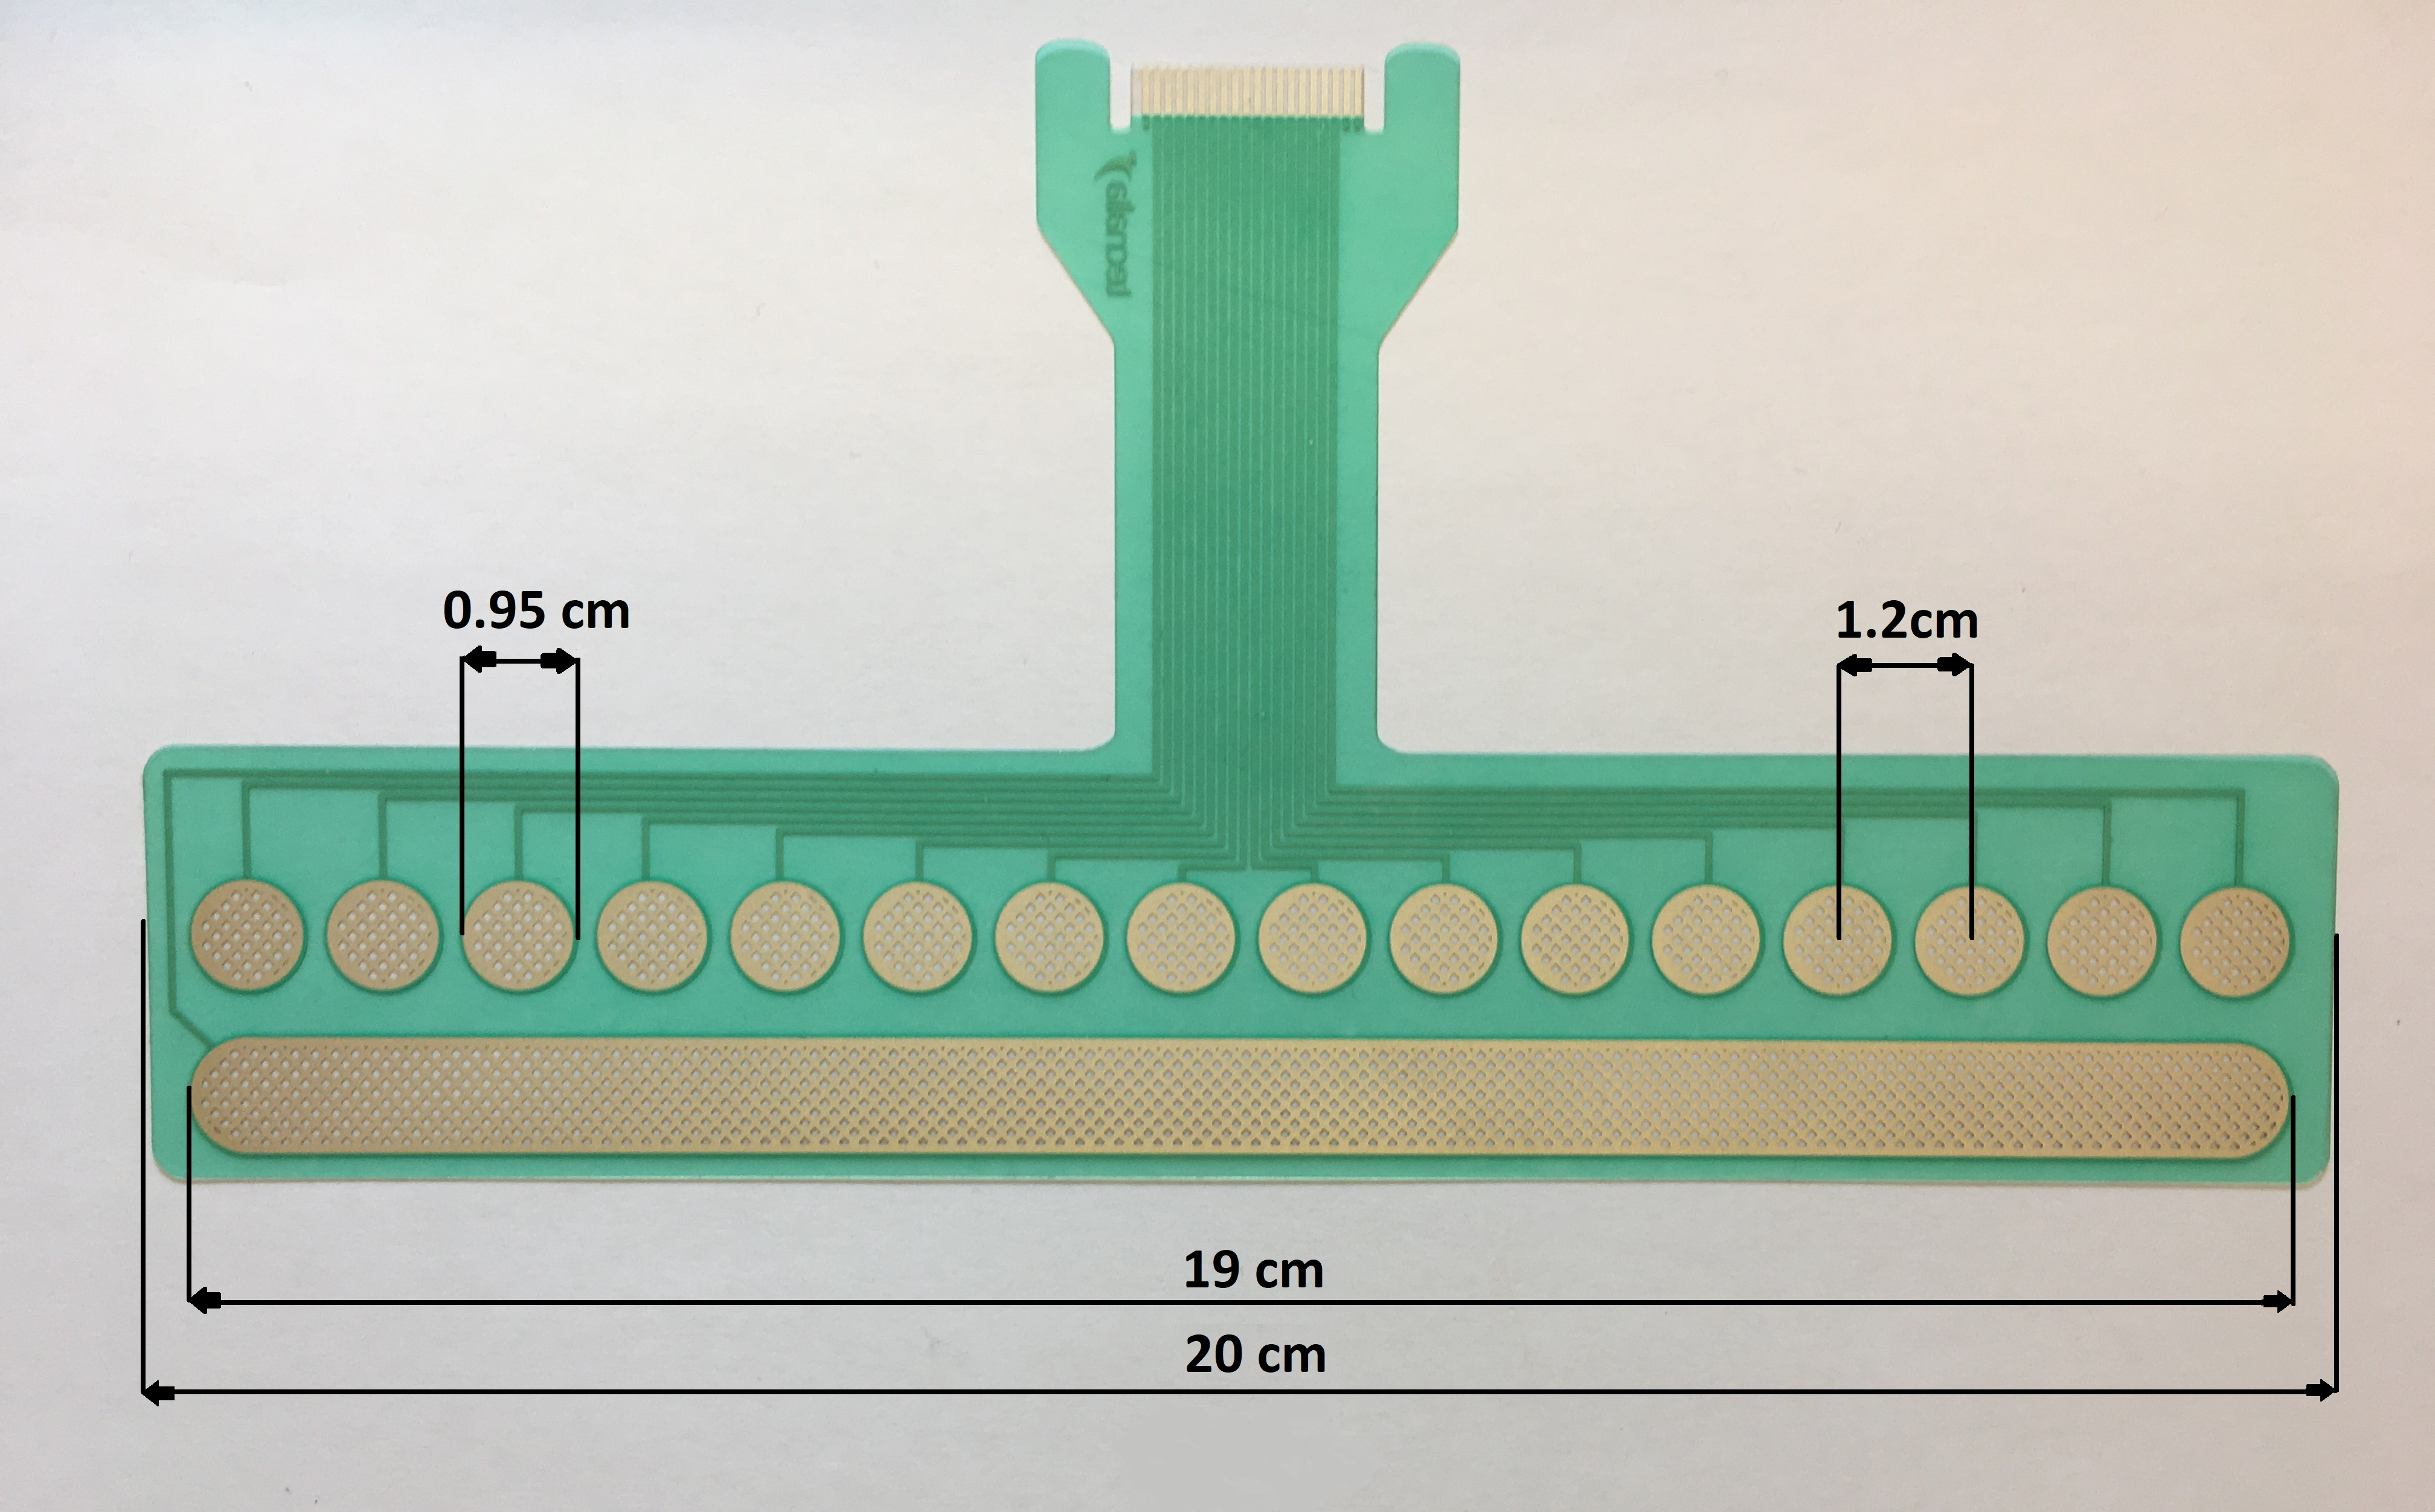
\includegraphics[width=1\textwidth]{figures/electrode}  
	\caption{Image of the 16 multi-pad electrode array used for stimulation. It consisted of 16 circular cathode pads, which each shared a common anode.}
	\label{fig:pa:electrode} 
\end{figure}
\begin{figure}[h]                 
	\includegraphics[width=1\textwidth]{figures/max}  
	\caption{The MaxSense stimulation device used for independently controlling the activation of each pad in the attached electrode array.}
	\label{fig:pa:max} 
\end{figure}   
The array electrode consisted of a single anode pad and 16 circular cathode pads. The pads comprised of conductive Ag/AgCl traces imprinted in a 150 $\mu$m thick polyester layer. All pads were covered with conductive hydrogel (AG702, Axelgaard, Denmark) to enhance skin-electrode contact.  A multichannel stimulation feedback device (MaxSens, Tecnalia, Spain), seen in figure \ref{fig:pa:max}, generating biphasic pulses was connected to a standard desktop PC for individual control of pad activation. The pulse width and amplitude could be modulated independently for each pad whereas the frequency was controlled globally. The pulse width could be modulated within a 50 - 1000 $\mu $s range with 10 $\mu $s steps, frequency ranges from 1 - 400 Hz with 1 Hz steps and current amplitude ranges from 50 - 10000 $\mu $A with 0.1 $\mu $A steps. The array electrode was placed circumferentially around the non-dominant arm to avoid interference with the EMG electrodes, which were fitted on the dominant arm. In a clinical application both interfaces should be placed on the same arm (residual limb). The stimulation electrodes were fitted such that the end pads had a maximum gap of 3 cm centrally on the volar side, when using a pronated arm as reference position. Hence, how distal the electrode array was placed towards the wrist depended on the diameter of the subject's forearm. The following sections will present the two developed feedback configurations. 


\subsubsection{Spatial configuration}

The motivation behind the spatial configuration was to communicate wrist rotation by spatially rotating dorsally placed active electrode pads and to communicate hand aperture by changing activation between volarly placed pads. 
This feedback design was chosen in order to intuitively mimic the directions of the motions in the included DoF's. An illustration of the spatial configuration can be seen in figure \ref{fig:pa:spatial}. The pads were divided into two groups each responsible for conveying information about a single DoF. The dorsally placed pads were allocated for wrist rotation and the volarly placed for hand aperture. The pads were furthermore paired such that each pair would represent one of four intervals of the feedback variable. For wrist rotation the pads were connected in side by side pairs. For right-handed subjects the activation of pad pairs would rotate laterally when increasing rotational states during supination and rotate medially during pronation. For the hand aperture DoF the pairs consisted of oppositely located pads on the medial and lateral sides. When increasing aperture states the active pairs would move volarly and the distance between active pads would become shorter. When both feedback variables were active, the pads pairs corresponding to the level of the hand aperture and rotational angle would be activated. Thus, a maximum of four pads could be active simultaneously. The reason for grouping adjacently placed pads to convey information about the rotational DoF was to improve sensation perception by stimulating a larger skin area, as shown in Dosen et al. \cite{Dosen2015}. 
\begin{figure}[h]                 
	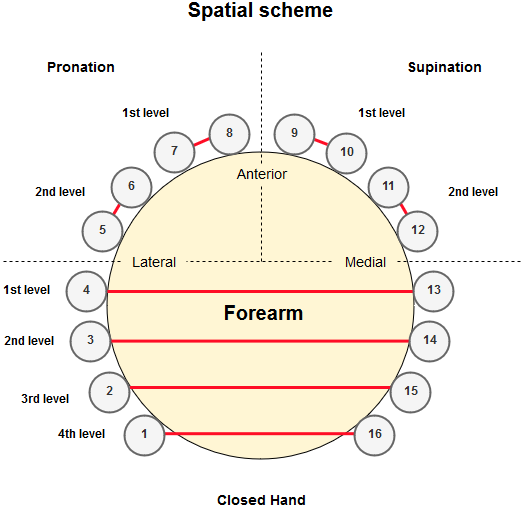
\includegraphics[width=.9\textwidth]{figures/El_array_spatial}  
	\caption{Transverse view of the developed spatial scheme fitted on the left arm of a subject. The levels written next to the pads pairs corresponded to the level of the position state; the higher the level, the higher the position state of the given movement was. When fitted on the right arm medial and lateral sides were reversed.}
	\label{fig:pa:spatial} 
\end{figure}   

\subsubsection{Amplitude configuration}
The incentive behind the amplitude configuration was to convey information by increasing the amplitude as the feedback variable increased. The feedback was provided in electrode pad groups of four.
The areas of active pads allocated for the various motions was similar to the spatial configuration to intuitively resemble the prosthesis motions. An illustration of the amplitude configuration can be seen in figure \ref{fig:pa:amplitude}. 
 \begin{figure}[h]                 
	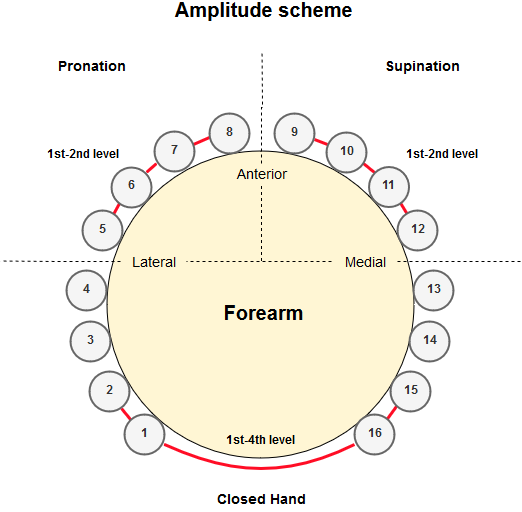
\includegraphics[width=.9\textwidth]{figures/El_array_amplitude}  
	\caption{Transverse view of the developed amplitude scheme fitted on the left arm of a subject. Different groups of four electrode pads were active during supination, pronation and hand aperture, respectively. The amplitude of the active pads would increase with the increase of the position state; the higher the position state level the higher the current amplitude of the given pads. When fitted on the right arm medial and lateral sides were reversed.}
	\label{fig:pa:amplitude} 
\end{figure}

The eight most dorsally placed pads were used for wrist rotation and the four most volarly placed pads for hand aperture. The eight pads used during wrist rotation were split such that the four most laterally placed were used during supination and four most medially placed were used during pronation for right-handed subjects. The pad activation was reversed for left-handed subjects. As the position state of a given movement would increase the current amplitude in the pads corresponding to that movement would increase. When in combined DoF position states, the pads corresponding to the level of the position state of each DoF would be active in the relative amplitude level. Thus, a maximum of eight pads could be active concurrently. The choice of grouping four electrode pads was decided upon to exploit the highest number of pads in the electrode array, while maintaining a symmetric distribution of possible active pads. Similarly to the spatial configuration this design was chosen to improve sensation perception \cite{Dosen2015}.


